\documentclass{beamer}

\mode<presentation> {
	
	% The Beamer class comes with a number of default slide themes
	% which change the colors and layouts of slides. Below this is a list
	% of all the themes, uncomment each in turn to see what they look like.
	
	%%%\usetheme{default}
	%\usetheme{AnnArbor}
	%\usetheme{Antibes}
	%\usetheme{Bergen}
	%\usetheme{Berkeley}
	%\usetheme{Berlin}
	%%%\usetheme{Boadilla}
	%\usetheme{CambridgeUS}
	%\usetheme{Copenhagen}
	%%%\usetheme{Darmstadt}
	%%%\usetheme{Dresden}
	%%%\usetheme{Frankfurt}
	%\usetheme{Goettingen}
	%\usetheme{Hannover}
	%\usetheme{Ilmenau}
	%\usetheme{JuanLesPins}
	%\usetheme{Luebeck}
	%\usetheme{Madrid}
	%\usetheme{Malmoe}
	%%%\usetheme{Marburg}
	%%%\usetheme{Montpellier}
	%\usetheme{PaloAlto}
	%\usetheme{Pittsburgh}
	\usetheme{Rochester}
	%\usetheme{Singapore}
	%\usetheme{Szeged}
	%\usetheme{Warsaw}
	
	% As well as themes, the Beamer class has a number of color themes
	% for any slide theme. Uncomment each of these in turn to see how it
	% changes the colors of your current slide theme.
	
	%\usecolortheme{albatross}	
	%\usecolortheme{beaver}
	%\usecolortheme{beetle}
	%\usecolortheme{crane}
	%\usecolortheme{dolphin}
	%\usecolortheme{dove}
	%\usecolortheme{fly}
	%\usecolortheme{lily}
	%\usecolortheme{orchid}
	%\usecolortheme{rose}
	%\usecolortheme{seagull}
	\usecolortheme{seahorse}
	%\usecolortheme{whale}
	%\usecolortheme{wolverine}
	
	%\setbeamertemplate{footline} % To remove the footer line in all slides uncomment this line
	\setbeamertemplate{footline}[page number] % To replace the footer line in all slides with a simple slide count uncomment this line
	
	\setbeamertemplate{navigation symbols}{} % To remove the navigation symbols from the bottom of all slides uncomment this line
}


\usepackage[utf8]{inputenc}
\usepackage[ukrainian]{babel}

\usepackage[active]{srcltx}
\usepackage[final]{pdfpages}

\usepackage{amssymb}
\usepackage{physics}
\usepackage{verbatim}
\usepackage{graphicx} % Allows including images
\usepackage{booktabs} % Allows the use of \toprule, \midrule and \bottomrule in tables

\numberwithin{equation}{section}

%------------------------------------------------
% custom commands

\newcounter{e}
\setcounter{e}{0}
\newcommand{\n}{\refstepcounter{e} (\arabic{e})}

\newcounter{pic}
\setcounter{pic}{0}
\newcommand{\pic}[1]{\refstepcounter{pic} \vspace{-0.3cm}\textit{Рисунок \arabic{pic}\label{#1}.}}

\newcounter{tabl}
\setcounter{tabl}{0}
\newcommand{\tabl}[1]{\refstepcounter{tabl} \vspace{-0.3cm}\textit{Таблиця \arabic{tabl}\label{#1}.}}

\numberwithin{equation}{section}
\numberwithin{figure}{section}

\newcommand{\tran}{^{T}}
\newcommand{\ith}{^{(i)}}
\newcommand{\lth}{^{(l)}}

\newcommand{\tabboxl}[2]{\parbox{#1}{\vspace{0.1cm} #2 \vspace{0.1cm} }}

\newcommand{\tabboxr}[2]{\parbox{#1}{\vspace{-0.3cm}
		\begin{flushright} #2 \end{flushright} \vspace{-0.3cm} }}

\newcommand{\tabboxc}[2]{\parbox{#1}{\vspace{-0.3cm}
		\begin{center} #2 \end{center} \vspace{-0.3cm} }}

%------------------------------------------------
\usepackage[
backend=biber,
style=numeric,
sorting=none
]{biblatex}
\addbibresource{../resources/bibliography.tex}

\nocite{ongie2020deep}
\nocite{Goodfellow-et-al-2016}
\nocite{Adler_2017}
\nocite{NIPS2012_6cdd60ea}

%------------------------------------------------
%	TITLE PAGE
%------------------------------------------------

% The short title appears at the bottom of every slide, the full title is only on the title page
\title[Short title]{Використання глибокого навчання для обернених задач} 

 % Your name
\author{Середович Віктор}

 % Your institution as it will appear on the bottom of every slide, may be shorthand to save space
\institute[UCLA]
{
	Львівський національний університет імені Івана Франка \\
	Факультет прикладної математики та інформатики 
}

% Date, can be changed to a custom date
\date{\today}

\begin{document}
	%------------------------------------------------
	
	\begin{frame}
		\titlepage
	\end{frame}
	
	\begin{frame}
		\frametitle{Зміст}
		\tableofcontents 
	\end{frame}
	
	%------------------------------------------------
	\section{Постановка задачі} 
	%------------------------------------------------
	\begin{frame}
		\frametitle{Постановка задачі}
		
		Оберненими задачами будемо вважати такі задачі, в яких невідомим є $n-\text{піксельне }$ зображення $\boldsymbol{x} \in \mathbb{R}^{n}$ яке було отримане з $m$ вимірювань $\boldsymbol{y} \in \mathbb{R}^{m}$ відповідно до рівняння \ref{eq:forward-problem}.
		\begin{block}{Загальне подання оберненої задачі}
			\begin{equation}
				\label{eq:forward-problem}
				\boldsymbol{y}=\mathcal{A}\left(\boldsymbol{x}\right)+\boldsymbol{\varepsilon}
			\end{equation}
		\end{block}
		де $\mathcal{A}$ - це прямий оператор вимірювання та $\boldsymbol{\varepsilon}$ є певним вектором шуму.
	\end{frame}
	%------------------------------------------------
	\section{Структура обернених задач}	
	\begin{frame}
		\frametitle{Структура обернених задач}
		\begin{block}{Задача максимальної ймовірності (maximum likelihood)}
			\begin{equation}
				\label{eq:ML-problem}
				\hat{\boldsymbol{x}}_{\mathrm{ML}}
				= \arg \max_{\boldsymbol{x}} {p (\boldsymbol{y} | \boldsymbol{x})}
				= \arg \min_{\boldsymbol{x}} -\log p(\boldsymbol{y} | \boldsymbol{x})
			\end{equation}
		\end{block}
		де $p(\boldsymbol{y} \mid \boldsymbol{x})$ це ймовірність спостереження $\boldsymbol{y}$ за умови якщо $\boldsymbol{x}$ є справжнім зображенням.
		
		\begin{block}{Задача для випадку білого гаусівського шуму }
			\begin{equation}
				\label{eq:MAP-avgn}
				\hat{x}=\arg \min_{x} 	\frac{1}{2}\|\mathcal{A}(\boldsymbol{x})-\boldsymbol{y}\|_{2}^{2}+\lambda 	\mathrm{R}(\boldsymbol{x})
			\end{equation}
		\end{block}
		де, $\mathrm{R}(\boldsymbol{x})$ - член регуляризації, а $\lambda$ є параметром регуляризації.
		
	\end{frame}
	%------------------------------------------------
	\section{Автоенкодер для розв'язування обернених задач}
	\subsection{Автоенкодер}
	\begin{frame}
		\frametitle{Автоенкодер}
		
		\begin{figure}[H]
			\centering
			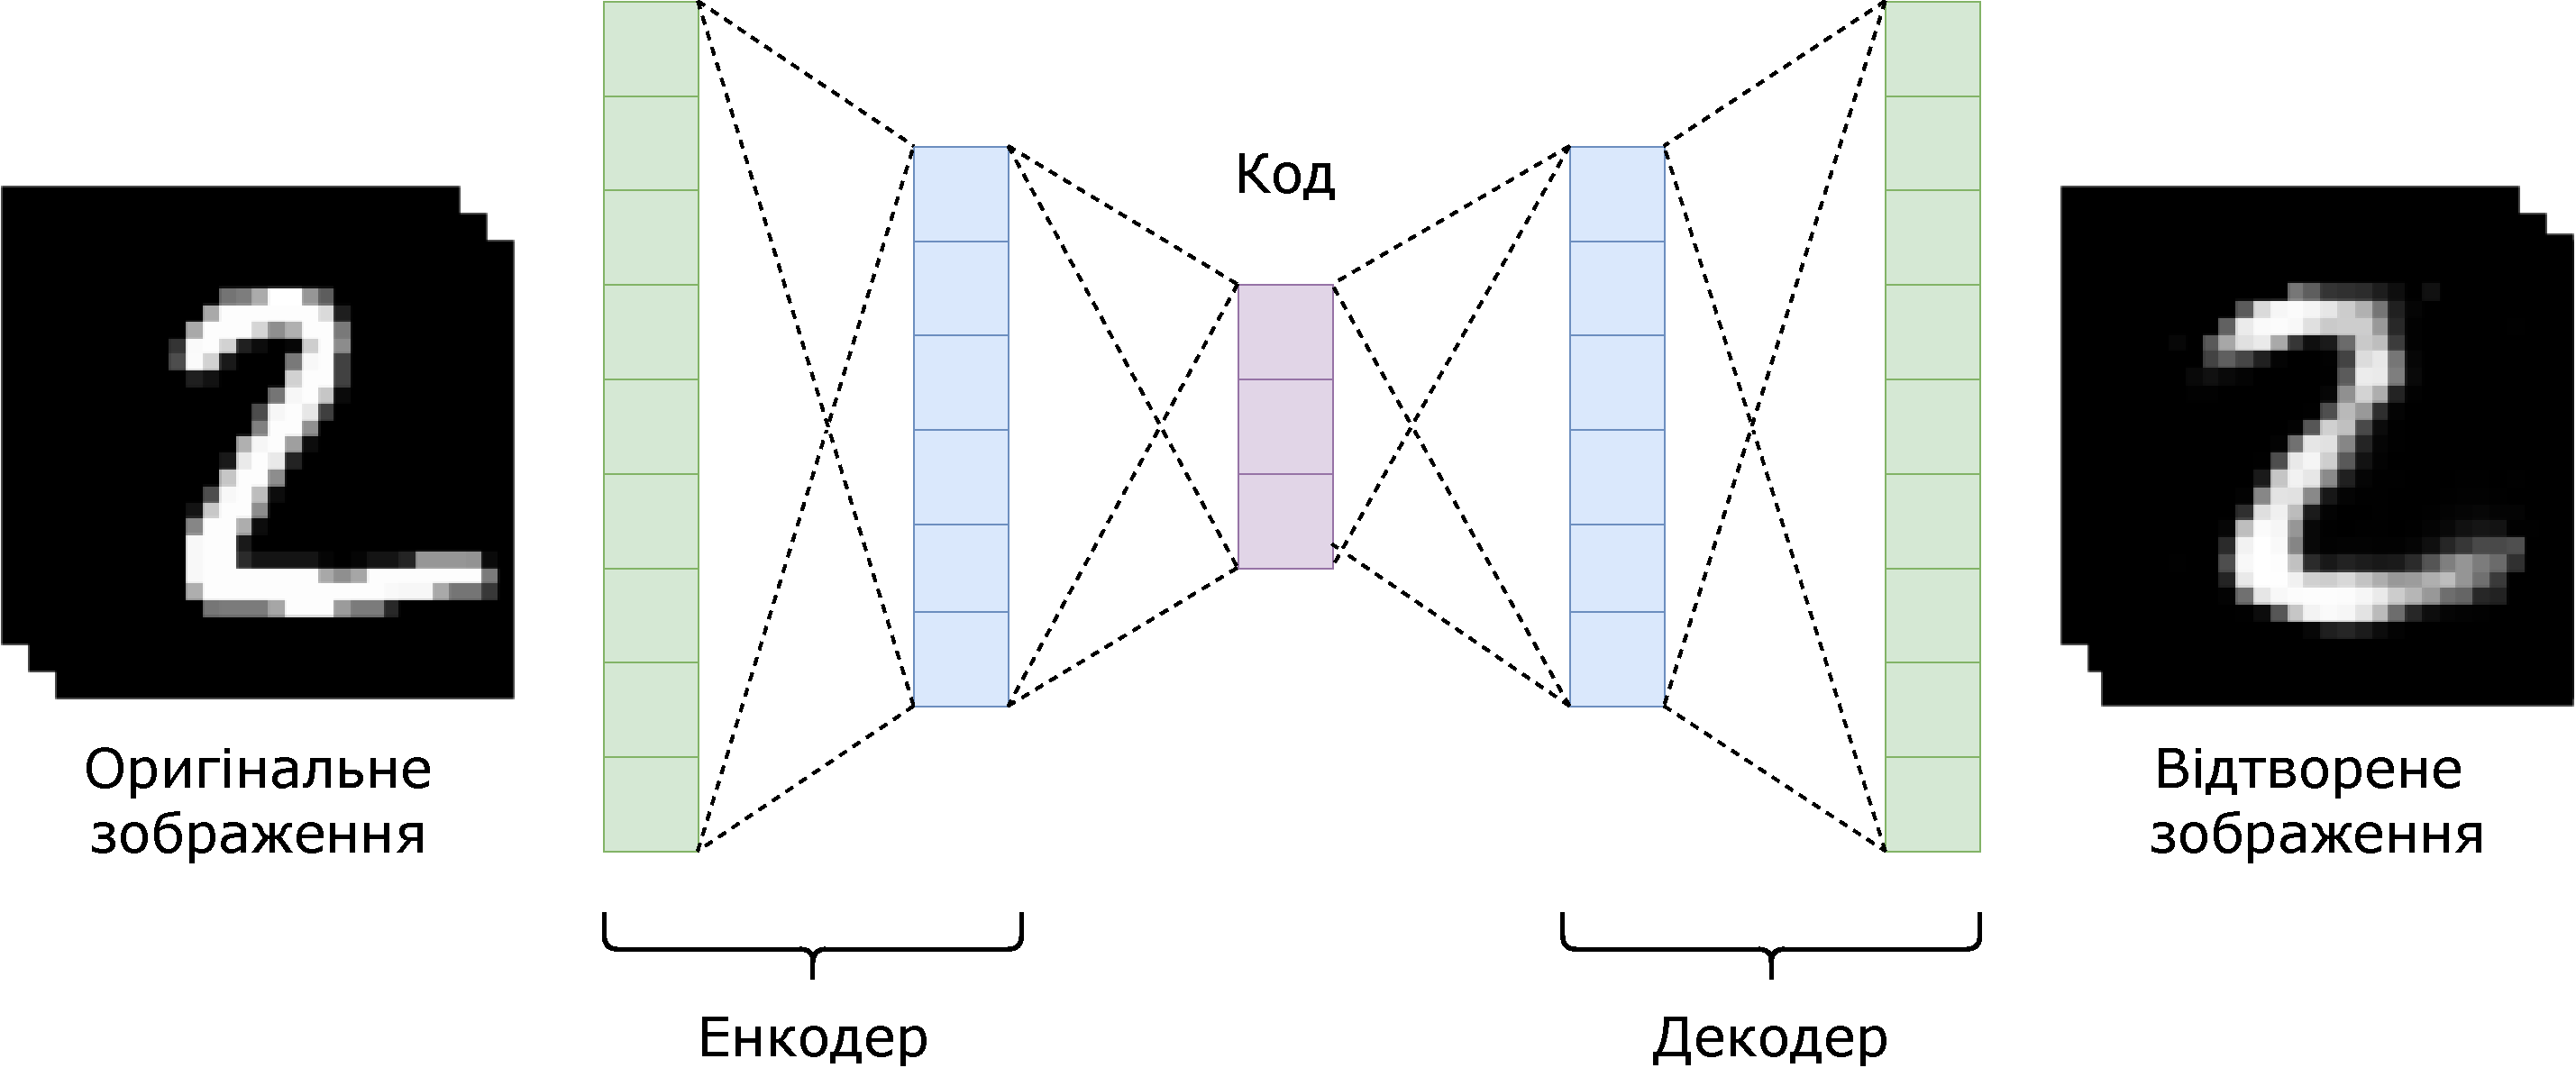
\includegraphics[width=1\textwidth]{../resources/autoencoder.pdf}
			\label{fig:autoencoder}
			\caption{Загальна структура автоенкодера, що відображає "оригінальне зображення"\ на "відтворене зображення"\ через внутрішнє представлення "код". }
		\end{figure}
	\end{frame}

	\subsection{Автоенкодер для видалення шуму}
	\begin{frame}
		\frametitle{Автоенкодер для видалення шуму}
		
		\begin{figure}[H]
			\centering
			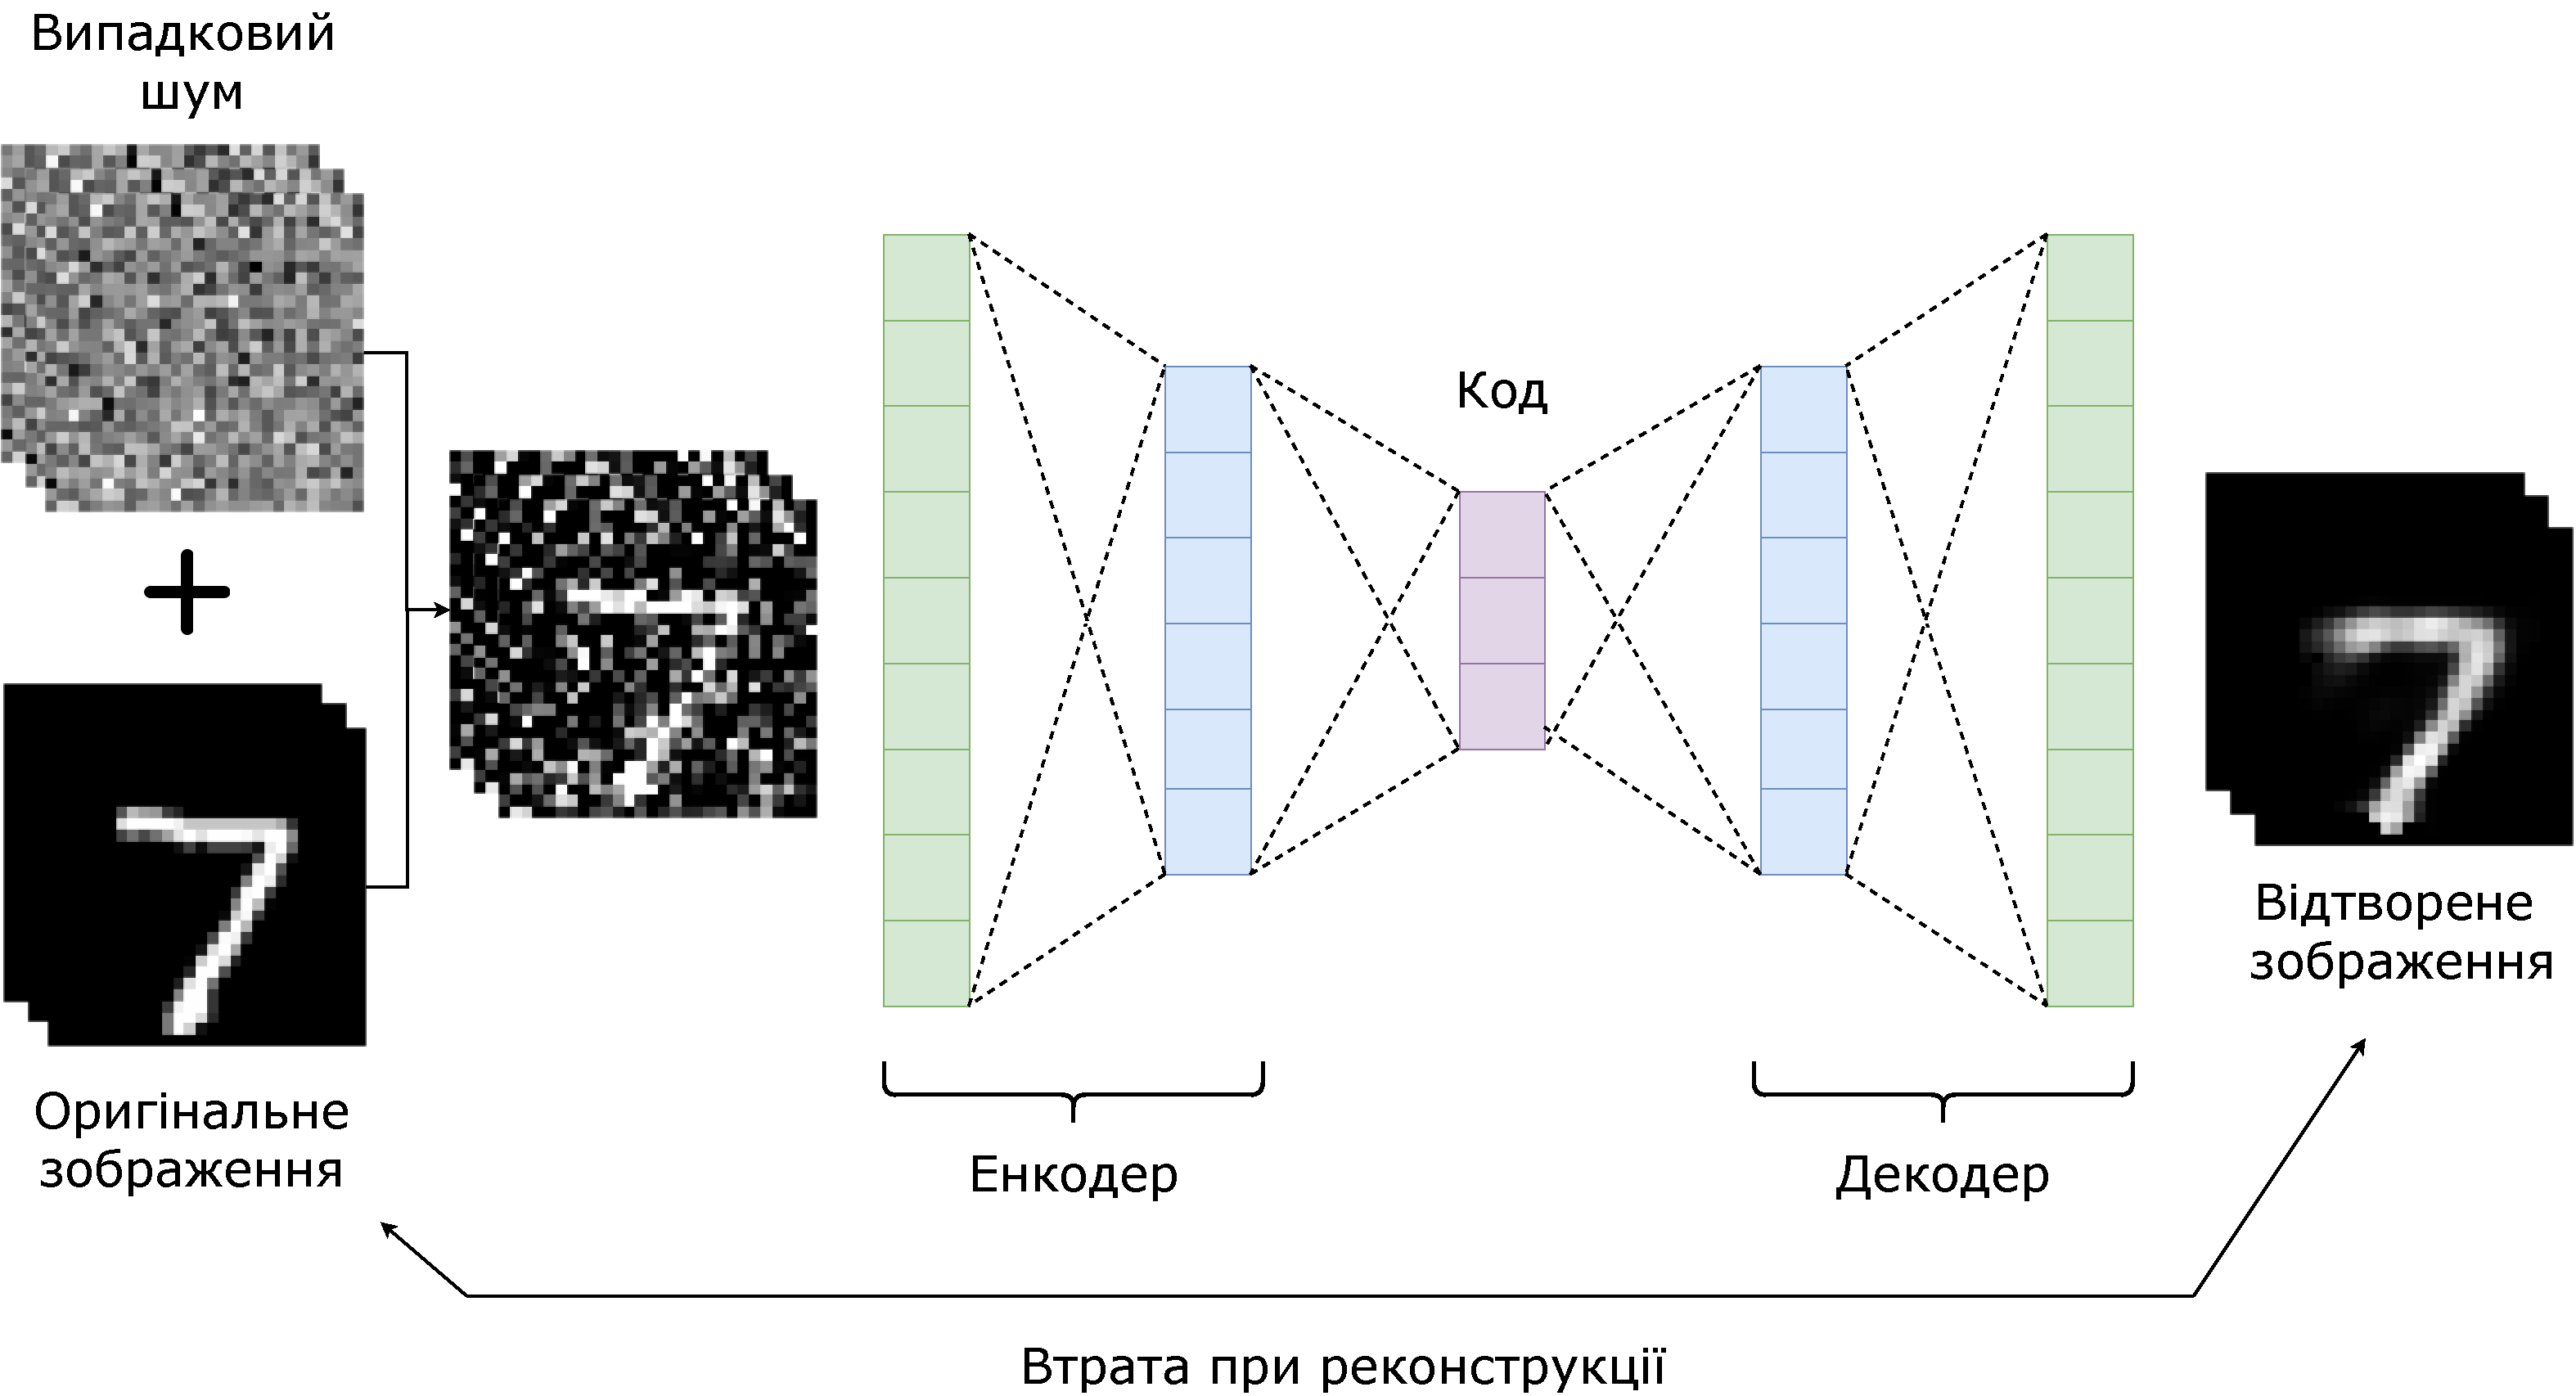
\includegraphics[width=1\textwidth]{../resources/dae.pdf}
			\caption{
				Структура функції витрат для автоенкодера який навчається реконструювати оригінальні зображення $x$ з пошкоджених деяким випадковим шумом.}
			\label{fig:danoising-autoencoder}
		\end{figure}
	\end{frame}
	%------------------------------------------------
	\section{Реалізація моделі для автоенкодера}

	\subsection{Оцінка реконструкції}
	\begin{frame}
		\frametitle{Оцінка реконструкції}
		\begin{block}{MSE штрафна функція}
			\begin{equation}
				\label{eq:cost-function}
				J(\omega, b) =  \frac{1}{m}  \sum_{i=1}^{m} L(a^{(L, i)}, y\ith)
			\end{equation}
		\end{block}
		\begin{block}{Функція втрати для одного набору елементів за $L_2$ нормою}
			\begin{equation}
				\label{eq:loss-function}
				L(a^{(l, i)}, y\ith)  =  \frac{1}{2}  \| a^{(l, i)}  - y\ith \|_{L_2}^{2} = \frac{1}{2} \sum_{j=1}^{n}  (a^{(l, i)}_j -  y\ith_j)^2
			\end{equation}
		\end{block}
	\end{frame}
	
	%------------------------------------------------
	\subsection{Оцінка зображень}
	\begin{frame}
		\frametitle{Оцінка зображень}
		\begin{block}{SSIM (structural similarity index measure) оцінка зображень.}
			\begin{equation}
				\label{eq:SSIM}
				\operatorname{SSIM}(x, y)=\frac{\left(2 \mu_{x} \mu_{y}+c_{1}\right)\left(2 \sigma_{x 			y}+c_{2}\right)}{\left(\mu_{x}^{2}+\mu_{y}^{2}+c_{1}\right)\left(\sigma_{x}^{2}+\sigma_{y}^{2}+c_{2}\right)}
			\end{equation}
		\end{block}
		де
		\begin{itemize}
			\item $\mu_{x}$, $\mu_{y}$  середнє значення $x$, $y$
			\item $\sigma_{x}^{2}$, $\sigma_{y}^{2}$ дисперсія $x$, $y$
			\item $\sigma_{x y}$ коваріація $x$ та $y$
			\item $c_{1}=\left(k_{1} L\right)^{2}, c_{2}=\left(k_{2} L\right)^{2}$
			\item $L$ - динамічний діапазон пікселів
			\item $k_{1}=0.01$ та $k_{2}=0.03$ - константи.	
		\end{itemize}
	\end{frame}
	
	\subsection{Архітектура моделі для автоенкодера}
	\begin{frame}
		\frametitle{Архітектура моделі для автоенкодера}

	Була побудована модель автоенкодера, яка задана таблицею \ref{tab:autoencoder-model}.
		\begin{center}
			\begin{table}[!htbp]
				\centering
				\begin{tabular}{|c|c|}
					\hline \tabboxc{6cm}{Шар мережі (активаційна функція)}
					& \tabboxc{4cm}{Розмірність} \\
					
					\hline \multicolumn{2}{|c|}{\tabboxc{2cm}{Енкодер}} \\
					
					\hline \tabboxc{4cm}{Dense (Relu)}
					& $784 \times 64$ \\
					
					\hline \tabboxc{4cm}{Dense (Relu)}
					& $64\times 32$ \\
					
					\hline \multicolumn{2}{|c|}{\tabboxc{2cm}{Декодер}} \\
					
					\hline \tabboxc{4cm}{Dense (Sigmoid)}
					& \tabboxc{3cm}{$32\times784$}\\
					\hline
				\end{tabular} 
				\caption{Архітектура щільної нейронної мережі для автоенкодера.}
				\label{tab:autoencoder-model}
			\end{table}
		\end{center}
	\end{frame}

	\subsection{Тренування}
	\begin{frame}
		\frametitle{Тренування}
		
		\begin{figure}[H]
			\centering
			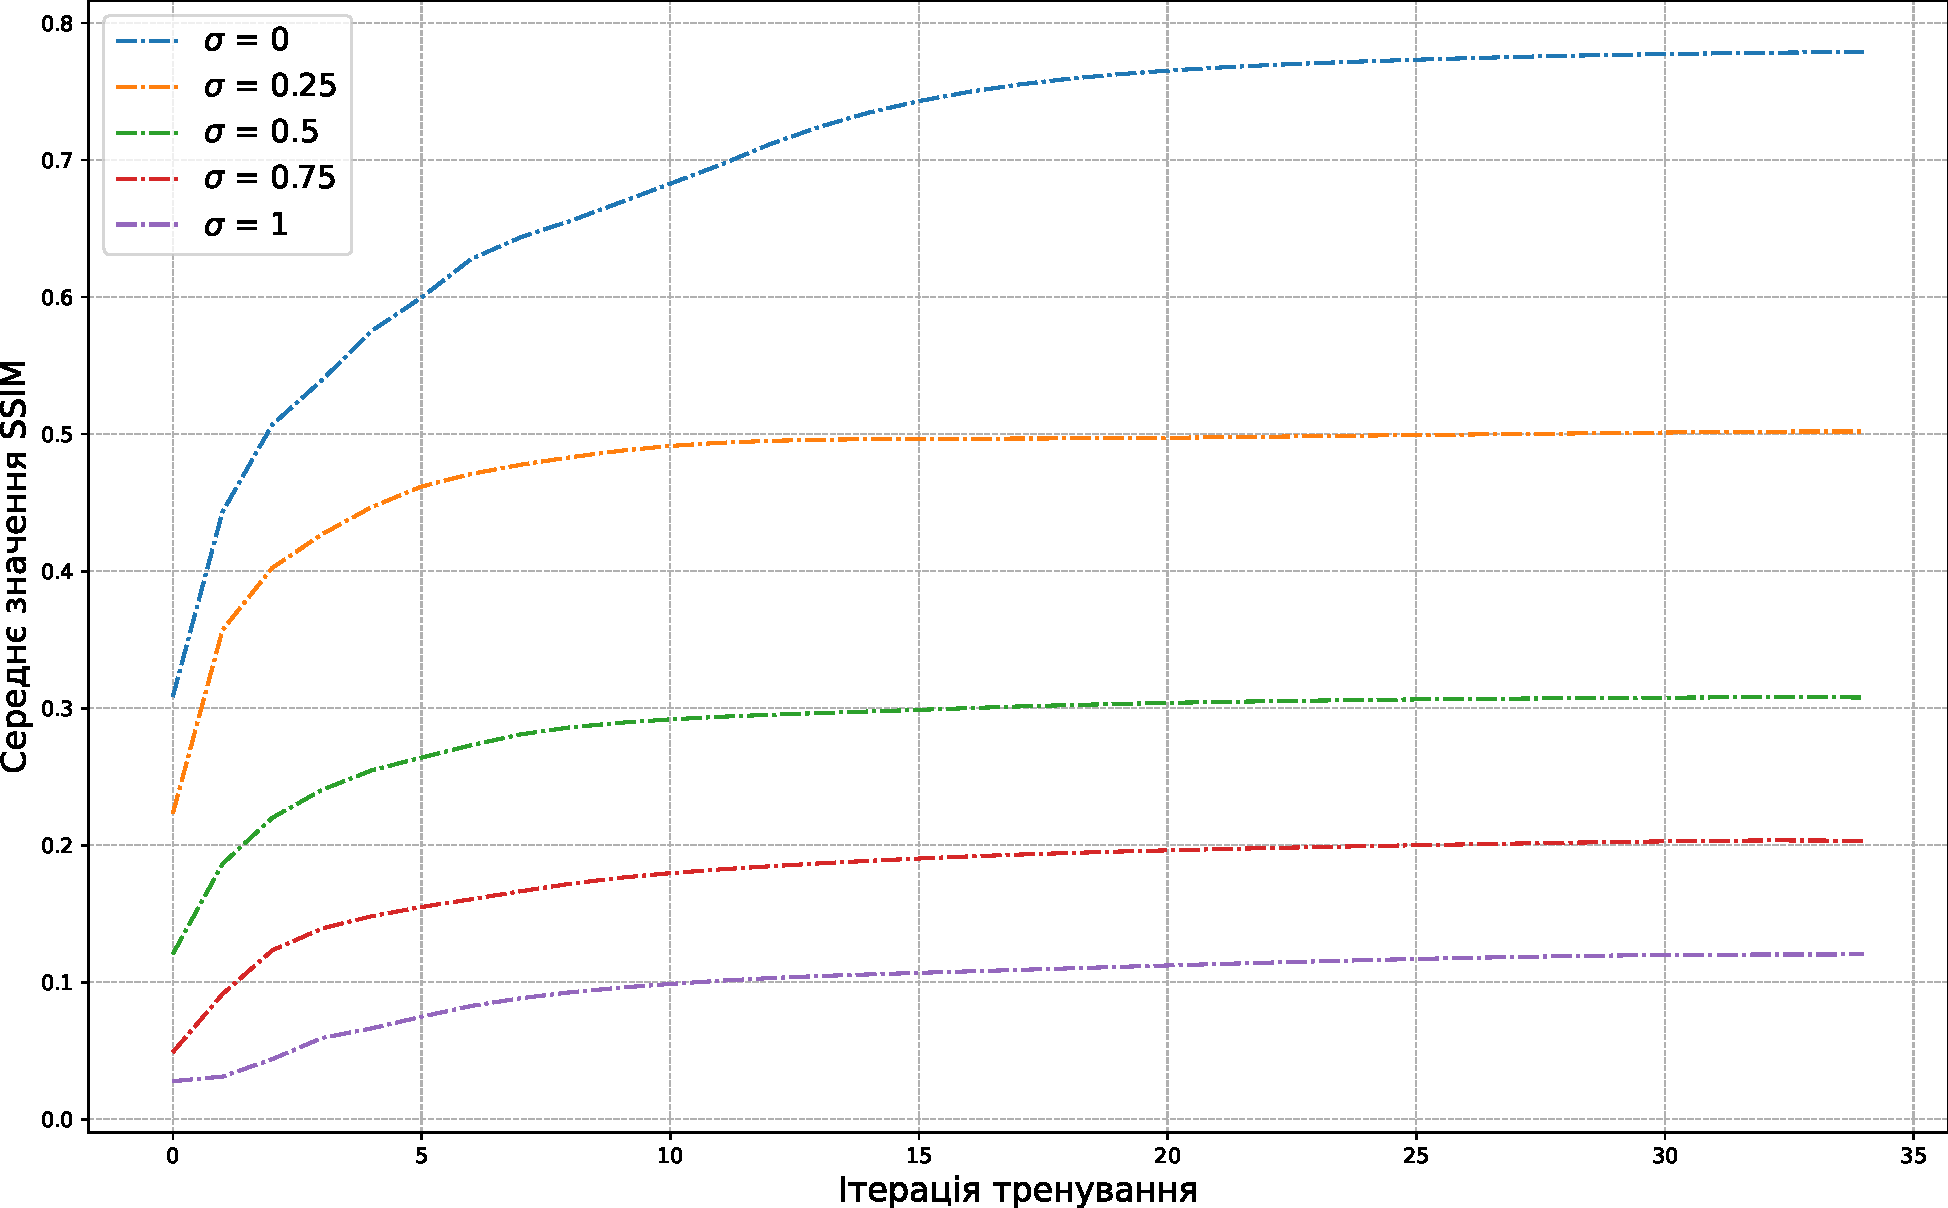
\includegraphics[width=0.8\textwidth]{../resources/awgn-train-ssim-comparation.pdf}
			\caption{Графік залежності усередненої SSIM оцінки для тестового датасету від кількості ітерацій тренування. $\sigma$ відповідає стандартному відхиленню гаусівського шуму.}
			\label{fig:awgn-train-ssim-comparation}
		\end{figure}
	\end{frame}

	%------------------------------------------------
	\section{Аналіз результатів}
		
	\begin{frame}
		\frametitle{Результати роботи автоенкодера для видалення}
		
		\begin{figure}[H]
			\centering
			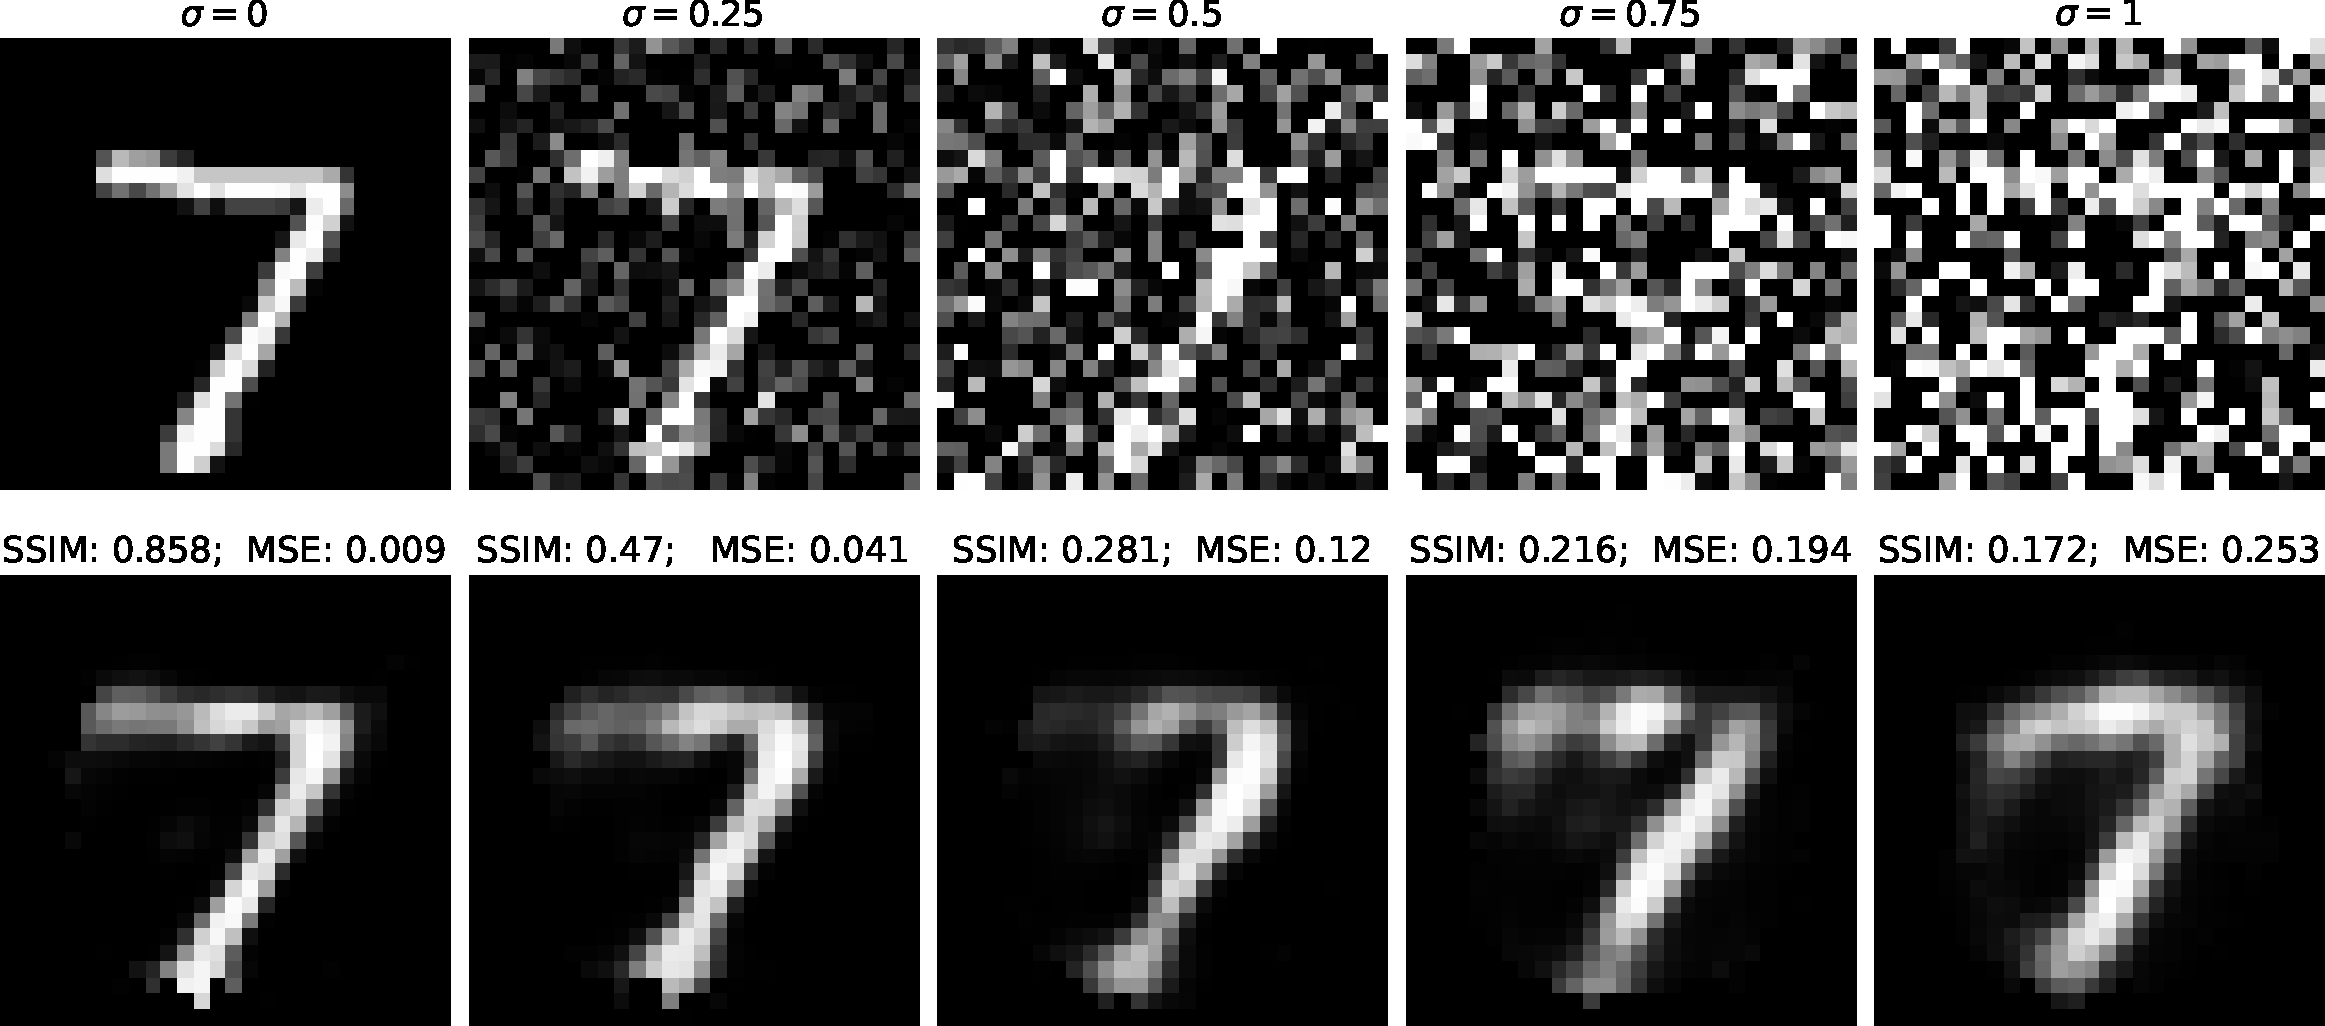
\includegraphics[width=1\textwidth]{../resources/denoising-awgn-comparation.pdf}
			\caption{Порівняння точності реконструкції зображень автоенкодером для різної величини стандартного відхилення $\sigma$ білого шуму.}
			\label{fig:denoising-awgn-comparation}
		\end{figure}
	\end{frame}

	\begin{frame}
		\frametitle{Порівняння роботи автоенкодера з регуляризацією}
		\begin{figure}[H]
			\centering
			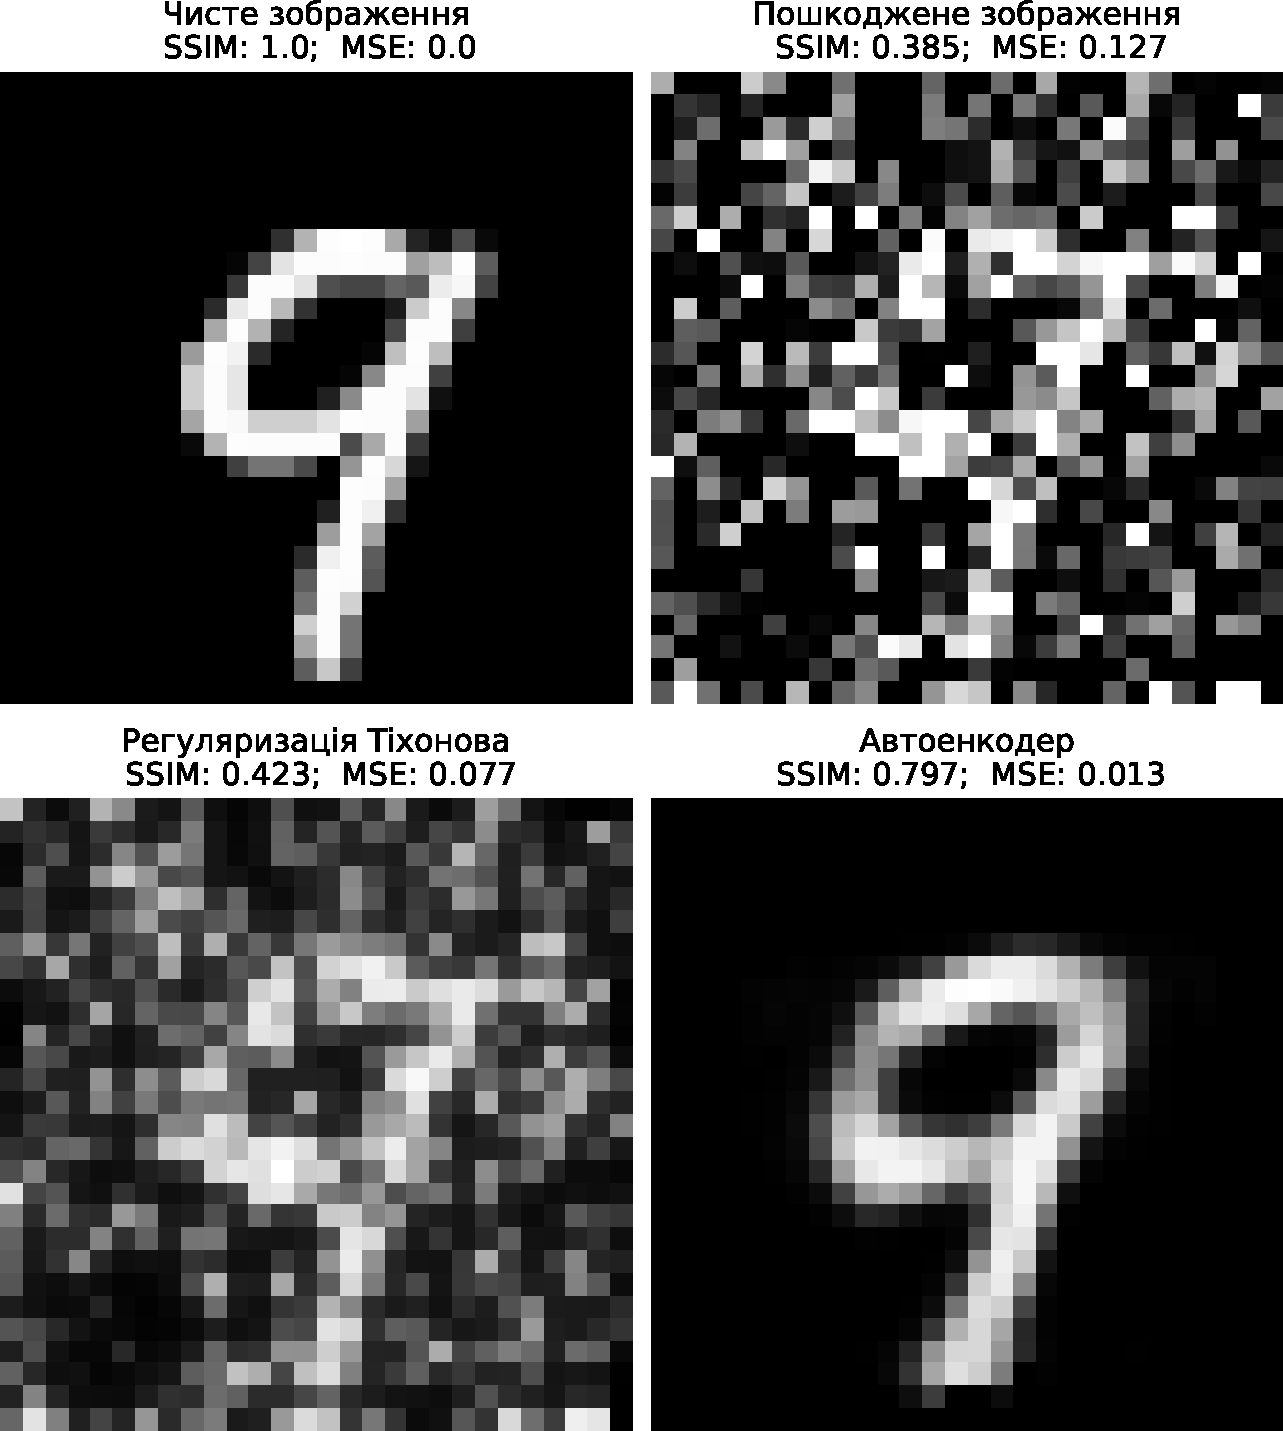
\includegraphics[width=0.5\textwidth]{../resources/denoising-methods-comparation.pdf}
			\caption{Порівняння видалення шуму за допомогою автоенкодера з класичним методом основаним на регуляризації.}
			\label{fig:denoising-methods-comparation}
		\end{figure}
	\end{frame}
	%------------------------------------------------
	\section{Висновок}	
	\begin{frame}
		\frametitle{Висновок}
		За результатами експериментів можна сказати, що побудована модель глибокого навчання є досить ефективною у розв'язанні розглянутої оберненої задачі. Вона успішно впоралась з видаленням шуму при його низьких показниках та дала прийнятні результати для його надмірної кількості. Варто зазначити, що автоенкодер продемонстрував себе значно краще в порівнянні з методом регуляризації. Можна стверджувати що використання глибокого навчання для розв'язання поставленої обернених задачі по видаленню шуму є ефективним підходом.
	\end{frame}
	%------------------------------------------------
	\begin{frame}
		\printbibliography[title={Література}]
	\end{frame}
	
	%------------------------------------------------
	
\end{document} 